\documentclass[fleqn,10pt]{wlpeerj}
\title{Large, structurally-curated alignment and phylogeny of Vertebrate biogenic amine receptors}

\author[1,2,3]{Stephanie J. Spielman}
\author[4,5]{Ahmad R. Sedaghat}
\author[1,2,3]{Keerthana Kumar}
\author[1,2,3]{Claus O. Wilke}
\affil[1]{Department of Integrative Biology, The University of Texas at Austin, Austin, U.S.A.}
\affil[2]{Institute of Cellular and Molecular Biology, The University of Texas at Austin, Austin, U.S.A.}
\affil[3]{Center for Computational Biology and Bioinformatics, The University of Texas at Austin, Austin, U.S.A.}
\affil[4]{Department of Otolaryngology–Head and Neck Surgery, Massachusetts Eye and Ear Infirmary, Boston, Massachusetts, U.S.A.}
\affil[5]{Department of Otology and Laryngology, Harvard Medical School, Boston, Massachusetts, U.S.A.}

\keywords{biogenic amine receptors, phylogenetics, multiple sequence alignment, G-protein coupled receptors}

\begin{abstract}
Amine receptors are important, and alignments are really hard. Here, we make a really large and structurally aware alignment of these receptors and demonstrate its use in phylogenetic reconstruction. Phylogeny made with structural information is dramatically superior to alignment not specifically curated for structural consensus. We are also able to identify both misclassified and previously unclassified receptors. You should use our alignment to do whatever studies you want. 
\end{abstract}

\begin{document}

\flushbottom
\maketitle
\thispagestyle{empty}

\section*{Introduction}

In spite of these receptors’ biological and clinical importance, studies on their evolution are limited. A broad phylogeny of all human GPCR paralogs has shown that HRHs belong to the clade of Rhodopsin family GPCRs, along with the other bioamine GPCRs (e.g. receptors for dopamine, serotonin, or adrenaline) (Fredriksson, Lagerstrom et al. 2003)
Like all members of the GPCR family, HRHs contain seven transmembrane domains separated by three extracellular (ECL) and three intracellular (ICL) loops, and propagate intracellular signaling through a G protein-mediated pathway.  

one of the most diverse membrane protein gene families in Metazoa, the G protein-coupled receptor (GPCR) family. GPCRs are the frequent targets of structural and biochemical studies; over 40\% of pharmaceuticals target GPCRs, and a multitude of diseases are caused by mutant GPCRs \citep{Dorsam2007,Schoneberg2004,Kristiansen2004,Fredriksson2003}. Phylogenetic analyses have shown that GPCRs form five main families, with the vast majority of human receptors belonging to the Rhodopsin-like (Family A) clade \citep{Fredriksson2003,Fredriksson2005}. Owing to their enormous diversity of biological functions and the ongoing expansion of their ligand repertoire, GPCRs have been described as one of the most evolutionarily successful gene families \citep{Bockaert1999,Lagerstrom2008}. Although protein sequences among, and indeed within, GPCR families are widely divergent, all GPCRs share a common structure characterized by a N-outside C-inside orientation with seven TM alpha helices spanning the plasma membrane, separated by three intracellular and three extracellular loops. 

Here, we focus on one of the most pharmaceutically-relevant GPCR groups: the bioamine receptors. These receptors include dopaminergic, serotonin, histamine, trace, adrenergic, and cholinergic, and their various subtypes.

GPCRs accept a wide variety of ligands, both endogenous (e.g.\ hormones, amines, or ions) and exogenous (e.g.\ odorants), and facilitate signal transduction through a G protein mediated pathway \citep{Kristiansen2004,Lagerstrom2008,Rosenbaum2009}.
Although some larger ligands do bind the extracellular portion of GPCRs, nearly all family A GPCRs, as well as many members of other GPCR families, bind ligands within their TM \citep{Vaidehi2002,Kristiansen2004,Bywater2005,Surgand2006,May2006,Park2008}. The notable expections to this trend are family C GPCRs, whose ligand-binding domains lie primarily in their extensive and diverse N-termini \citep{May2006,Park2008,Lagerstrom2008}. However, allosteric  modulators acting on all GPCR families bind within the TM. This commonality highlights the key role that the TM plays in the regulation of protein activity \citep{May2006,Lagerstrom2008}.

The TM domain is also a critical determinant of a GPCR's conformational state. Mutational studies have shown that altering specific residues in GPCR TM spans results in structural modifications that induce constitutive activity, regardless of ligand presence \citep{Spalding1998,Lu2000}. Maintaining the integrity of TM structure and sequence, then, is necessary for GPCRs to function properly.




Alignments are really hard sometimes, and amine receptors are really important. Previous attempts to examine evolution of this family have fallen somewhat short. Efforts to make a phylogeny have been hampered by poor alignment quality and confounding signals of gene duplication. Some have tried to do syntenic analysis, but this sort of analysis can be misled by gene conversion and/or gene relocation. 
Amine receptors are members of the Rhodopsin (A) family of GPCRs. Like all GPCRs, 7TMs. Loop sizes typically vary among GPCRs, but the 7TM anchors it in the membrane. This unique and highly conserved property allows us to align properly! If we can determine which domain each position is in, we can generate far more robust alignments which pay specific attention to structure. As GPCR structures are so deeply conserved, we don't even need a crystal structure, but we have a really good HMM program which has been validated on real structures (spielman2013). This strategy does not require time-consuming alignment softwares which make use of actual crystal structure data. these programs are very computationally intensive and, for an alignemnt of over 3000 sequences, are rather unwieldy. 


We therefore provide a comprehensive, structurally-curated alignment of vertebrate amine receptors. All sequences in this alignment have been robustly verified as gpcrs. We present three versions of the alignment: naive (more sequences), an alignment for which sequences not properly aligned with domains have been culled (unreliable), and that last alignment, but where residues which do not agree with column consensus have been masked. Using these three MSAs, we create ML phylogenies, and show that ...

Alignments and phylogenies are available at claus wilke's website, and we make all code available at github.


\section*{Results}

\subsection*{Sequence Collection and Processing}
We collected sequences using PSIBLAST using 42 distinct human bioamine receptor seed sequences. Parameters for the PSIBLAST search were set as an e-value of $10^{-20}$, 5 iterations, and returned only sequences belonging to the refseq database. We discarded sequences with less than 25\% sequence identity to and/or a length difference above 50\% from the starting seed sequence. We additionally discarded sequences in which more than 1\% positions were ambiguous or which were annotated as either low-quality, pseudogene, and/or partial. Next, we employed the software GPCRHMM to determine more robustly whether each sequences was indeed a G-protein coupled receptor, and we discarded all sequences which were not unambiguously GPCRs, ultimately resulting in a final data set of 3464 sequences.


\subsection*{Sequence Alignment}
 
At this stage, we adopted an alignment strategy to ensure that the overarching GPCR 7TM structure was maintained in the aligned sequences. We began by assigning, for each protein sequence, each protein residue to a particular domain: extracellular, intracellular, and transmembrane. In previous works, we predicted GPCR structures using GPCRHMM, and we found that, for Rhodopsin-type GPCRs, these predictions were completely accurate. Therefore, we again used it here to determine each residue's domain using a cutoff of 0.5 posterior probability. We then used the strategy shown in FigX to iteratively align and cull any sequences which did not conform to the overall structure. We ended up with 3039 total sequences. In addition to this alignment, we additionally created a domain-masked alignment, wherein any residues which did not match the column's consensus domain were masked with a '?'. This resulting alignment represents the largest and most well-curated vertebrate bioamine receptor, and indeed GCPR, alignment of ever.


\subsection*{Phylogeny}


To demonstrate the utility of this alignment, we created several phylogenies. 
1. Regular alignment, no structurally curated (contains 3463 sequences)
2. Curated alignment, unmasked. Two partitions.
3. Curated alignment, unmaked. No parititions.
4. Curated alignment, masked. Two parititions.
5. Curated alignment, masked. No parititions.
All were done with the LG+F AA exchangeability matrix.

\section*{Conclusions}
Please feel free to use our alignment for evolutionary analysis of amine receptors, GPCRs, transmembrane domains. Also have great use for identifying motifs, possible pharmaceutical application.

















\section*{Acknowledgments}

Funded by NIH, army, probably.

%\bibliography{sample}


\section*{Figures and Tables}


\begin{figure}[htbp]
	\centerline{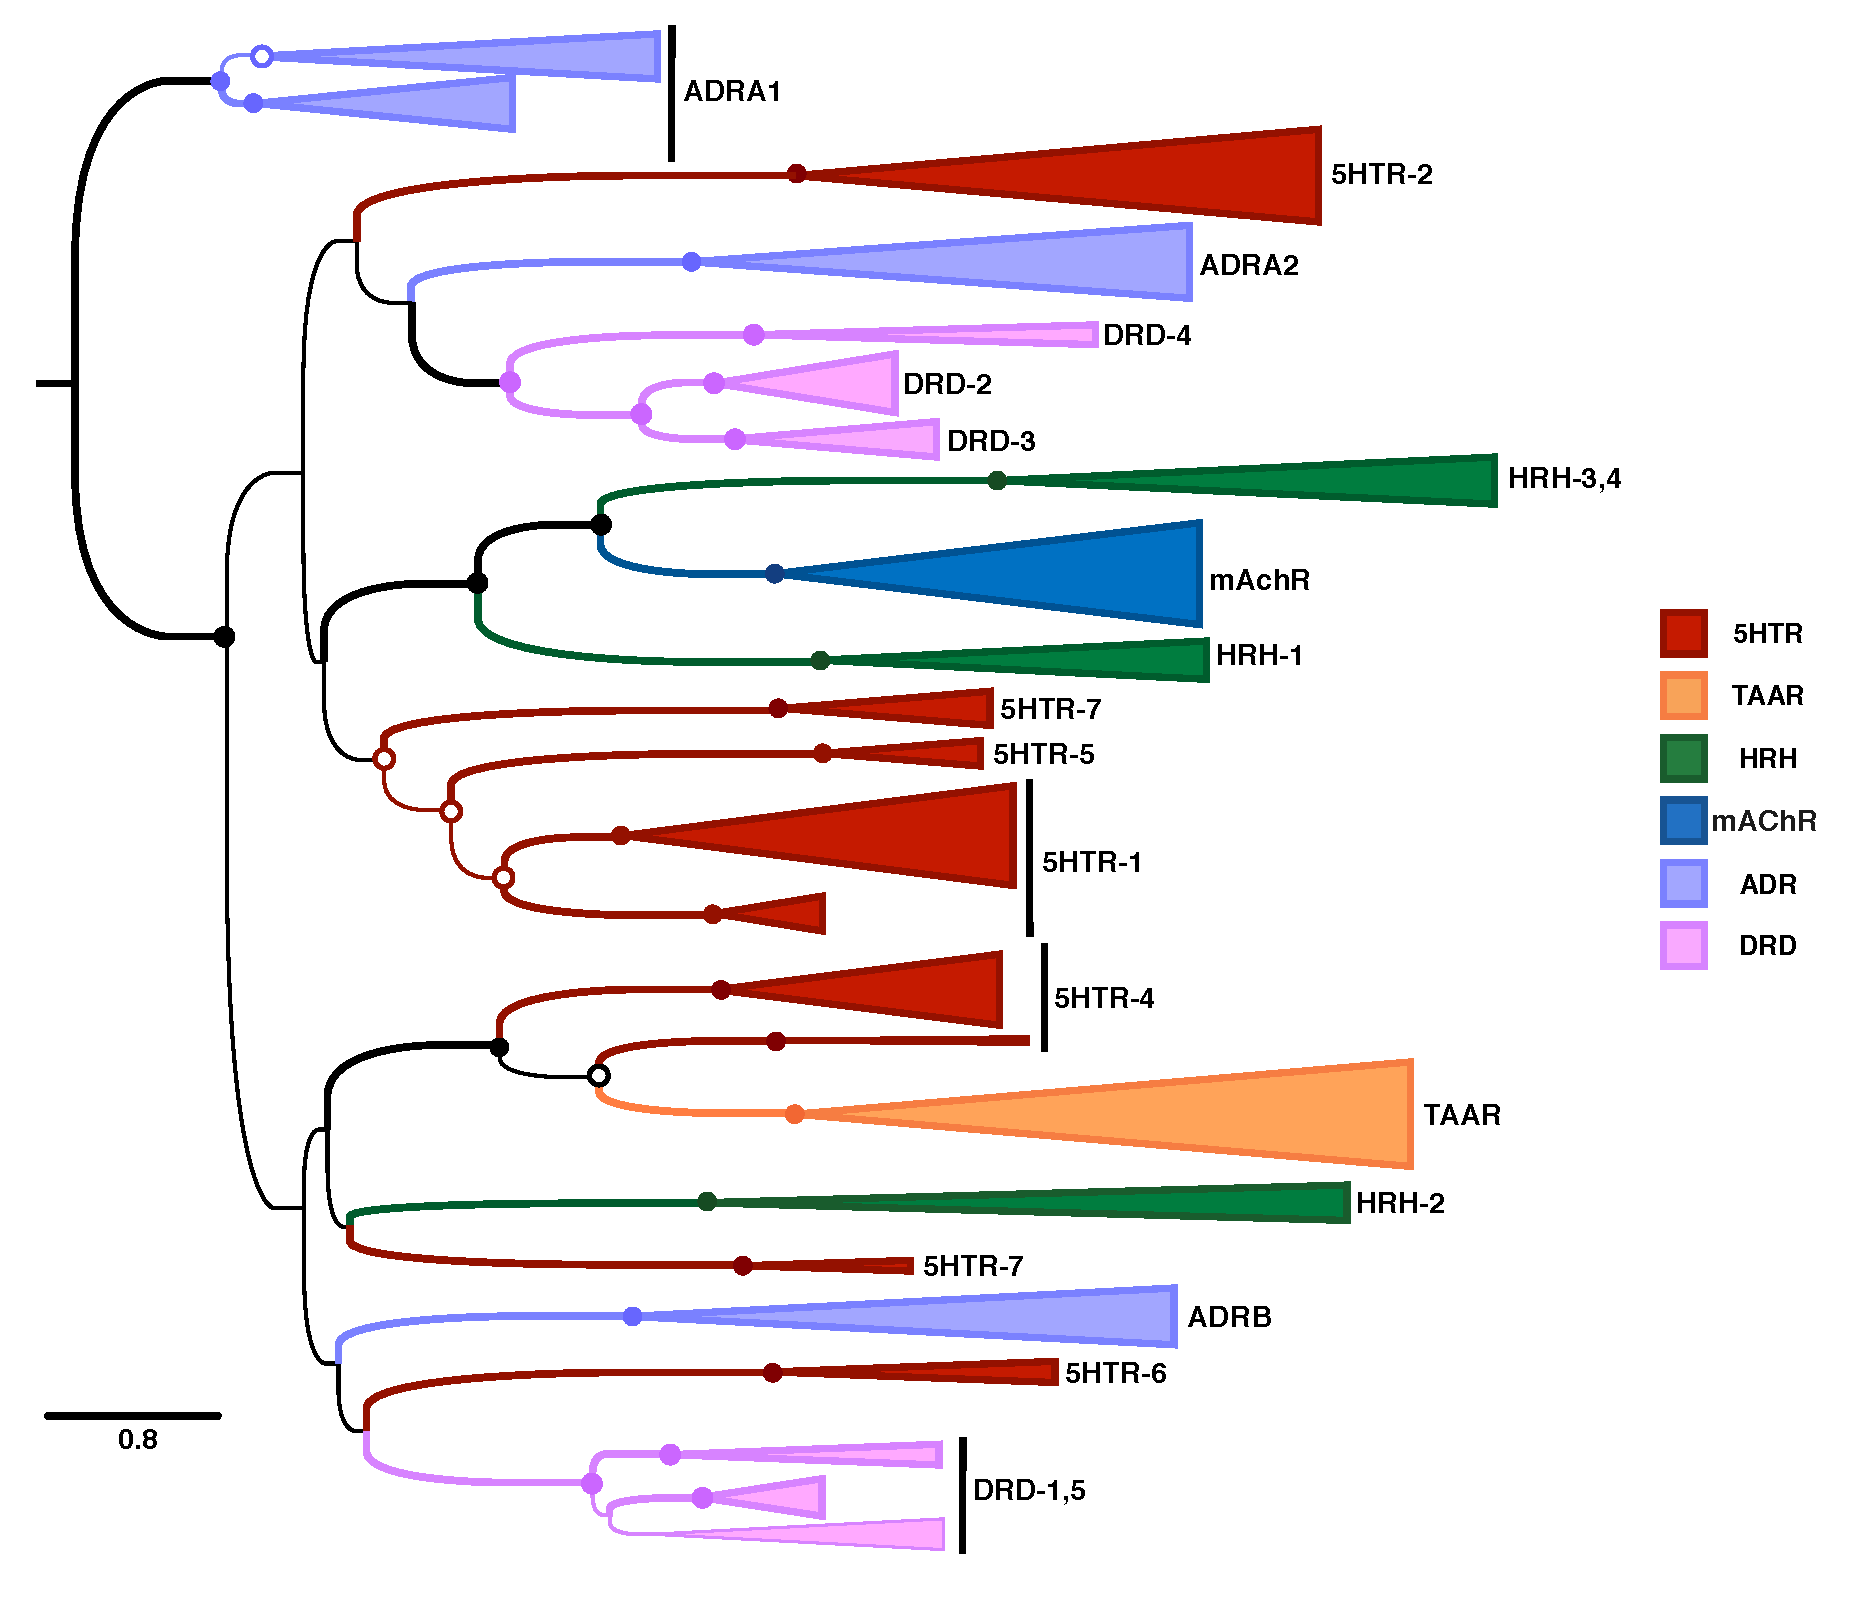
\includegraphics[width=18cm]{figures/masked_part_idraw.pdf}}
	\caption{\label{phylogeny} Maximum likelihood phylogeny of Vertebrate bioamine receptors built using the ``masked partitions'' alignment in RAxML. Nodes with open circles indicate $\geq 50\%$ bootstrap support, and nodes with closed circles and thick lines indicate $\geq 90\%$ bootstrap support. Bioamine receptors are abbreciated as 5HTR, serotonin receptors; TAAR, trace amine-associated receptors; HRH, histamine receptors; mAChr, muscarinic acetylcholine receptors; ADR, adreneric receptors; and DRD, dopamine receptors.}
\end{figure}








\end{document}